\chapter{PXE批量系统安装}
\label{chap:susePXE}

\section{PXE简介}
\label{sec:introPXE}

PXE(preboot execute environment)是由Intel公司开发的最新技术,工作
于Client/Server的网络模式,支持待安装服务器(Client)通过网络从远端安装
服务器(Server)下载映像,并由此支持来自网络的操作系统的启动安装过程,
其启动安装过程中,Client端要求安装服务器动态分配IP地址,再
用TFTP(Trivial File Transfer Protocol)或MTFTP(Multicast Trivial File
Transfer Protocol)协议下载一个启动软件包到本机内存中并执行,由这个启动
软件包完成Client端的基本软件设置,从而引导安装预先安装在安装服务器上
的Client端操作系统。

\section{PXE工作原理}
\label{sec:topoPXE}

\subsection{PXE工作原理框图}
\label{sec:processPXE}

\subsection{PXE工作原理示意图}
\label{sec:processPXEInstance}

\begin{figure}[hbtp]
\centering
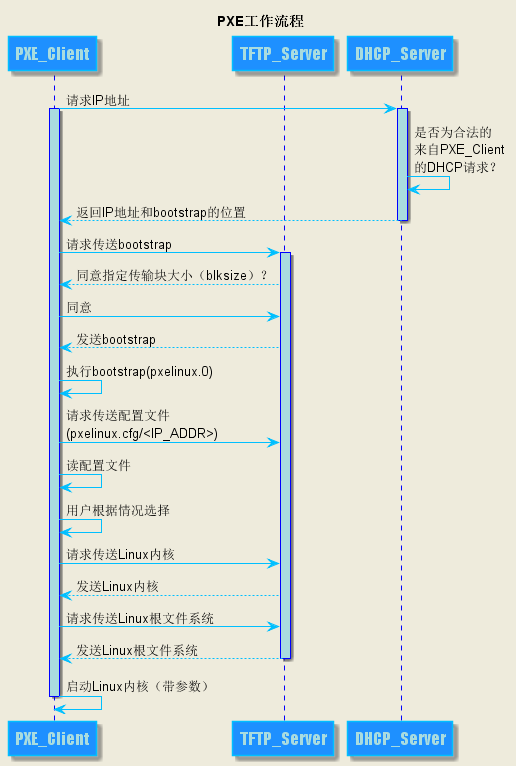
\includegraphics[width=.8\textwidth]{img/pxe01.png}
\caption{PXE工作原理示意图}
\end{figure}

工作原理示意图说明:
\begin{enumerate}[itemsep=0pt,parsep=0pt]
\item Client向PXE Server上的DHCP发送IP地址请求消息,DHCP检测Client是否
  合法(主要是检测Client的网卡MAC地址),如果合法则返回Client的IP地址,
  同时将启动文件pxelinux.0的位置信息一并传送给Client;
\item Client向PXE Server上的TFTP发送获取pxelinux.0请求消息,TFTP接收到
  消息之后再向Client发送pxelinux.0大小信息,试探Client是否满意,
  当TFTP收到Client发回的同意大小信息之后,正式向Client发送pxelinux.0;
\item Client执行接收到的pxelinux.0文件;
\item Client向TFTP发送针对本机的配置信息(记录在TFTP的pxelinux.cfg目录
  下),TFTP将配置文件发回Client,继而Client根据配置文件执行后续操作;
\item Client向TFTP发送Linux内核请求信息,TFTP接收到消息之后将内核文件发
  送给Client;
\item Client向TFTP发送根文件请求信息,TFTP接收到消息之后返回Linux根文件
  系统;
\item Client启动Linux内核(启动参数已经在4中的配置文件中设置好了);
\item Client通过NFS下载镜像文件,读取autoyast自动化安装脚本。至
  此,Client正式进入自动化安装模式开始安装系统直到完成。
\end{enumerate}

\section{开始搭建PXE服务器}
\label{sec:beginPXE}

PXE服务器包括DHCP服务、TFTP服务与NFS服务。PXE服务器安装完成后,配
置eth0的IP地址为192.168.241.1。其配置文件为:

\begin{verbatim}
# cat /etc/sysconfig/network/ifcfg-eth0
BOOTPROTO='static'
IPADDR='192.168.241.1/24'
STARTMODE='auto'
USERCONTROL='no'
\end{verbatim}

\subsection{安装及配置DHCP服务}
\label{sec:InstallDHCP}

安装DHCP服务端软件包,

\begin{verbatim}
# zypper install -y dhcp-server  
\end{verbatim}

配置DHCP服务端,修改/etc/dhcpd.conf配置文件,

\begin{verbatim}
# vi /etc/dhcpd.conf
max-lease-time 7200;
ddns-updates off;
ddns-update-style none;
default-lease-time 600;
subnet 192.168.241.0 netmask 255.255.255.0 { 
  option routers 192.168.241.254;
  next-server 192.168.241.1;
  filename "pxelinux.0";
  range 192.168.241.11 192.168.241.55;
  default-lease-time 14400;
  max-lease-time 172800;
}
host test1 {                                 
  hardware ethernet 30:30:30:30:30:30;
  fixed-address 192.168.241.11;
}  
\end{verbatim}

修改/etc/sysconfig/dhcpd配置文件,修改DHCPD\_INTERFACE的配置项,根据实
际情况修改,

\begin{verbatim}
DHCPD_INTERFACE="eth0"  
\end{verbatim}

之后,启动DHCP服务,

\begin{verbatim}
# service dhcpd start
# rcdhcpd status  
\end{verbatim}

\section{安装及配置TFTP服务}
\label{sec:InstallTFTP}

安装TFTP软件包,
\begin{verbatim}
# zypper install -y tftp  
\end{verbatim}

修改配置文件,内容如下,
\begin{verbatim}
# cat /etc/xinetd.d/tftp 
# default: off
# description: tftp service is provided primarily for booting or \
#   when a router need an upgrade. Most sites run this only on \
#   machines acting as "boot servers".
service tftp
{
    socket_type             = dgram
    protocol                = udp
    wait                    = yes
    flags                   = IPv6 IPv4
    user                    = root
    server                  = /usr/sbin/in.tftpd
    server_args             = -s /opt/pxe/tftpboot
    disable                 = no 
}  
\end{verbatim}

启动TFTP服务,

\begin{verbatim}
# service xinetd restart  
\end{verbatim}

\section{安装及配置NFS服务}
\label{sec:InstallNFS}

安装NFS服务端软件包,
\begin{verbatim}
# zypper install -y nfs-kernel-server  
\end{verbatim}

NFS服务配置,
\begin{verbatim}
# vi /etc/exports
/opt/pxe/iso *(ro,async)  
/opt/pxe/autoinst *(ro,async)
\end{verbatim}

启动NFS服务,
\begin{verbatim}
# rcnfsserver start  
\end{verbatim}

\section{SLEL11sp2系统镜像文件}
\label{sles11sp2Image}

\subsection{目录结构}
目录结构为表\ref{PxeDir}所示:
\begin{table}[hbtp]
  \centering
    \begin{tabular}{ll}
      \toprule
      目录           & 说明 \\
      \midrule
      /opt/pxe/iso       & 镜像文件SLES-11-SP2-DVD-x86\_64-GM-DVD1.iso放置目录 \\
      /opt/pxe/tftpboot  & tftp根目录 \\
      /opt/pxe/autoinst  & 自动化安装脚本autoyast放置目录 \\
      \bottomrule
    \end{tabular}
    \caption{PXE目录结构}\label{PxeDir}
\end{table}

\subsection{镜像挂载}

\begin{verbatim}
# mkdir -p /opt/pxe/iso
# mount -o loop SLES-11-SP2-DVD-x86_64-GM-DVD1.iso /opt/pxe/iso  
\end{verbatim}

\subsection{复制系统内核文件}

\begin{verbatim}
# mkdir -p /opt/pxe/tftpboot/pxelinux.cfg
# cp /usr/share/syslinux/pxelinux.0 /opt/pxe/tftpboot
# cp /usr/share/syslinux/menu.c32 /opt/pxe/tftpboot
# cp /opt/pxe/iso/boot/x86_64/loader/linux /opt/pxe/tftpboot
# cp /opt/pxe/iso/boot/x86_64/loader/initrd /opt/pxe/tftpboot
\end{verbatim}

\subsection{创建default文件}

\begin{verbatim}
PXEServer:~# cd /opt/pxe/tftpboot/pxelinux.cfg
PXEServer:~# vi default
default menu.c32
prompt 1
timeout 100
label local 
localboot 0   	
label linux
kernel linux
append initrd=initrd install=nfs://192.168.241.1/opt/pxe/iso \
autoyast=nfs://192.168.241.1/opt/pxe/autoinst/autoinst.xml \
splash=silent showopt  
\end{verbatim}

\subsection{AutoYast自动化安装脚本}

批量安装系统之前,首先手动安装一台PXE服务器,系统安装完成之后,
在/root/目录下生成一个autoinst.xml文件,即为自动化安装脚本。

\begin{verbatim}
# mkdir -p /opt/pxe/autoinst
# cp /root/autoinst.xml /opt/pxe/autoinst  
\end{verbatim}

注意:
\begin{enumerate}[itemsep=0pt,parsep=0pt]
\item 若autoinst.xml自动化安装脚本中存在下列代码,须将下列代码删除;
\item 下列代码会把错误的网卡信息写入
  到/etc/udev/rules.d/70-persistent-net.rules文件,在系统安装完成后自动
  获取IP地址过程中,导致网卡识别错误,系统获取不到IP地址;
\item 删除下列代码后,系统才能自动获取IP地址。
  \begin{verbatim}
  <net-udev config:type="list">
   	   <rule>
      	  <name>eth0</name>
       	  <rule>ATTR{address}</rule>
       	</rule>
  	  </net-udev>  
  \end{verbatim}
\end{enumerate}

保证PXE服务器和待安装服务器(Client)处于同一网络,在Client启动过程中根
据提示手动按F12使后者以PXE模式启动,即可完成无人值守的自动化安装。

%%% Local Variables:
%%% mode: latex
%%% TeX-master: t
%%% End:
